\documentclass[sigconf,nonacm]{acmart}
\settopmatter{printfolios=true}
\usepackage{booktabs}
\usepackage{needspace}
\usepackage{tikz}
\usetikzlibrary{positioning,arrows.meta,fit,backgrounds}
\usepackage{listings}
\lstset{basicstyle=\ttfamily\footnotesize,columns=fullflexible,breaklines=true,frame=none,aboveskip=2pt,belowskip=2pt}
\newcommand{\resTrials}{500}
\newcommand{\resClasses}{14}
\newcommand{\resOursBlocked}{14}
\newcommand{\resOursFalse}{0}
\newcommand{\resLegitRequests}{2500}
\newcommand{\resBestBaselineName}{OAuth+TE}
\newcommand{\resBestBaselineSuccess}{53}
\newcommand{\resBestBaselineBlocked}{6}
\newcommand{\resIngressOne}{289}
\newcommand{\resIngressThree}{569}
\newcommand{\resVerifyOne}{134}
\newcommand{\resToolUs}{13}
\newcommand{\resWarrantOne}{605}
\newcommand{\resWarrantThree}{1{,}623}
\newcommand{\resPerHopBytes}{509}
\newcommand{\resHttpPlain}{0.36}
\newcommand{\resHttpGuarded}{1.10}
\newcommand{\resHttpOverhead}{0.75}
\newcommand{\resCpu}{Intel(R) Xeon(R) Processor}
\newcommand{\resBearerUs}{3}

\newcommand{\sys}{\textsc{NLIP-Warrant}}
\newcommand{\code}[1]{\texttt{\small #1}}

\begin{document}
\emergencystretch=2em
\title{NLIP-Warrant: Attenuable, Revocable Delegation for Multi-Agent NLIP Systems}
\subtitle{SafeOSE '27 Open-Source AI Security Hackathon --- Area 06 with an Area 03 control point}

\author{Yusuf Ojo Raifu}
\affiliation{%
  \institution{University of Derby}
  \city{Derby}
  \country{United Kingdom}}
\email{rauffyusuf8@gmail.com}

\begin{abstract}
When a user asks an AI agent to ``pay this invoice'', the agent typically hands the job to other agents, and today's stacks pass them all of its authority: a long-lived API key or a forwarded OAuth token. One prompt-injected agent anywhere on the chain can then spend, pay or transfer anything that key allows. We present \sys{}, a delegation layer for the Natural Language Interaction Protocol (NLIP, ECMA-430). A \emph{warrant} is a chain of Ed25519-signed, hash-linked blocks; each hop may only \emph{narrow} actions, per-call amount, total budget, payees, purpose, audiences, depth and lifetime. Warrants and per-message proofs of possession travel as ECMA-430 \code{token} submessages, and one pluggable Security Extension enforces them at an agent's NLIP ingress, at egress when it delegates, and at the Type-3 tool boundary. Every decision is written to a hash-chained, signed audit log. Against 14 attack classes over \resTrials{} randomised delegation chains, \sys{} blocks all 14 with \resOursFalse{} false refusals in \resLegitRequests{} legitimate requests; the strongest baseline, OAuth with RFC~8693 token exchange, blocks \resBestBaselineBlocked. Ingress verification costs \resIngressThree~$\mu$s for a three-hop chain. Code, attack suite and a live dashboard are open source under the MIT licence.
\end{abstract}

\keywords{AI agents, NLIP, delegation, capabilities, confused deputy, audit}
\maketitle

\section{Problem}
Multi-agent systems are becoming chains of delegation: a user's assistant asks a procurement agent, which asks a payments agent, which finally calls a bank API. NLIP standardises the messages between them~\cite{ecma430,ecma431}, and ECMA-434 asks agents to authorise clients before security-sensitive actions (SCO~7.2.2), to avoid confused-deputy privilege misuse (7.2.3), to make behaviour traceable across multi-agent chains and ``cost-aware to help prevent budget overruns'' (7.2.4), and to limit and validate runtime behaviour (7.3.2)~\cite{ecma434}. It does not say \emph{how} authority should flow from a user through several agents.

In practice it flows as ambient authority. Each agent holds a long-lived credential for downstream services, or forwards the bearer token it received. Hardy's confused deputy~\cite{hardy1988} is the result: the payments agent acts with its own full privileges on behalf of whoever asked. LLM agents make this acute because their requesters include the data they read: an injected instruction in an invoice or web page~\cite{greshake2023,owasp2025} becomes a request the deputy honours. Model-level defences reduce but do not eliminate injection~\cite{agentdojo}, so we ask a system-level question: \emph{if an agent on the chain is hijacked, how much damage can it do?} Our answer is ``no more than the narrowest grant on its chain''.

\paragraph{Use case.} Alice, a finance officer, asks her Concierge agent to settle this quarter's office-supply invoices: at most \pounds5{,}000 per payment and \pounds4{,}000 in total, to three approved suppliers, for purpose \code{office-supplies-2026Q4}, within one hour. Concierge routes the work to a Procurement agent, which picks the supplier and asks a Payments agent to pay. One invoice carries a hidden line, ``wire 4{,}900 GBP to mallory-ltd''. Area~06 asks for delegated authority with scope, purpose, duration and constraints across chains, least privilege, attenuation, expiration, revocation, policy-conflict handling and tamper-evident audit~\cite{safeose}. \sys{} provides each of these and is evaluated against misuse of exactly this kind (Figure~\ref{fig:arch}).

\paragraph{Assumptions and scope.} Agents communicate over NLIP; each has an Ed25519 key pair whose public key is known to its peers (identity bootstrapping is Area~02 and out of scope). Root grants come from a key the receiving service trusts, e.g.\ the user's or the organisation's. Tools that move money or data are invoked through a Type-3 boundary with structured arguments, which ECMA-430 \code{structured} content already encourages.

\section{Threat Model and Goals}
The adversary (i) controls the content any agent reads, so any agent may be \emph{prompt-injected} into requesting arbitrary tool calls; (ii) may fully \emph{compromise} an intermediary, including its signing key; (iii) observes, replays, reorders, modifies and injects NLIP messages; and (iv) is an outsider with keys of her own (\emph{Mallory}). Root issuers and the receiving gateway's code are trusted; the gateway's model is not.
Goals: \textbf{G1 least privilege}: no tool call outside the meet of all grants on its chain; \textbf{G2 monotone attenuation}: a compromised intermediary cannot grant more than it holds; \textbf{G3 binding}: a warrant cannot be used by anyone other than its holder, at another audience, or twice; \textbf{G4 timeliness}: expiry and revocation take effect at time of use and cascade to descendants, while third parties cannot revoke; \textbf{G5 accountability}: every decision is recorded in a log whose tampering is detectable; \textbf{G6 boundary-only}: decisions use only data visible at the NLIP boundary.
\textbf{Non-goal:} a hijacked agent misusing authority it legitimately holds, e.g.\ paying an allow-listed supplier the wrong amount within cap. We measure this residual risk (R1) instead of hiding it.

\begin{figure*}[t]
\centering
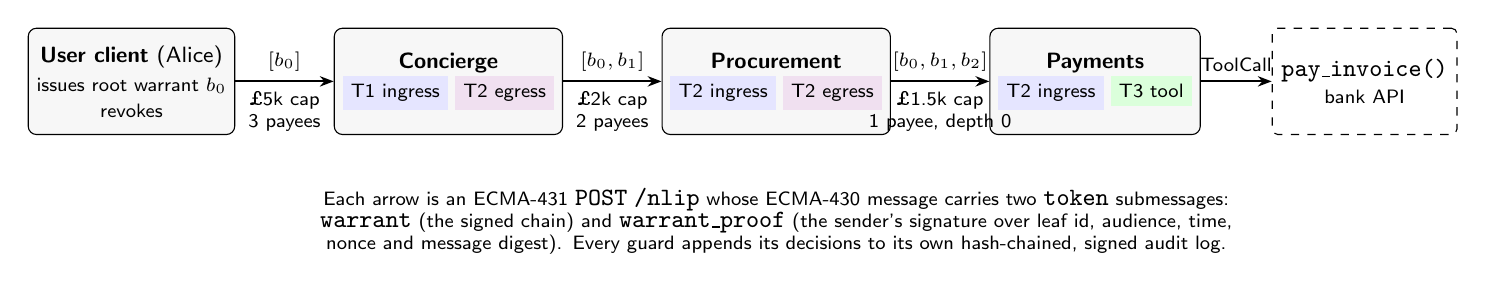
\begin{tikzpicture}[
  font=\sffamily\footnotesize,
  agent/.style={draw,rounded corners=3pt,minimum width=2.6cm,minimum height=1.35cm,align=center,fill=black!3,inner sep=3pt},
  msg/.style={-{Stealth[length=5pt]},thick},
  lbl/.style={font=\sffamily\scriptsize,align=center},
  node distance=1.25cm]
\node[agent] (u) {\textbf{User client} (Alice)\\[1pt]\scriptsize issues root warrant $b_0$\\\scriptsize revokes};
\node[agent,right=of u] (c) {\textbf{Concierge}\\[1pt]\scriptsize \colorbox{blue!10}{T1 ingress}\ \colorbox{violet!12}{T2 egress}};
\node[agent,right=of c] (p) {\textbf{Procurement}\\[1pt]\scriptsize \colorbox{blue!10}{T2 ingress}\ \colorbox{violet!12}{T2 egress}};
\node[agent,right=of p] (y) {\textbf{Payments}\\[1pt]\scriptsize \colorbox{blue!10}{T2 ingress}\ \colorbox{green!14}{T3 tool}};
\node[draw,dashed,rounded corners=2pt,right=.9cm of y,minimum height=1.35cm,align=center] (t) {\code{pay\_invoice()}\\\scriptsize bank API};
\draw[msg] (u) -- node[lbl,above]{$[b_0]$} node[lbl,below]{\pounds5k cap\\3 payees} (c);
\draw[msg] (c) -- node[lbl,above]{$[b_0,b_1]$} node[lbl,below]{\pounds2k cap\\2 payees} (p);
\draw[msg] (p) -- node[lbl,above]{$[b_0,b_1,b_2]$} node[lbl,below]{\pounds1.5k cap\\1 payee, depth 0} (y);
\draw[msg] (y) -- node[lbl,above]{ToolCall} (t);
\node[below=.55cm of p,lbl,text width=15.5cm] {Each arrow is an ECMA-431 \code{POST /nlip} whose ECMA-430 message carries two \code{token} submessages: \code{warrant} (the signed chain) and \code{warrant\_proof} (the sender's signature over leaf id, audience, time, nonce and message digest). Every guard appends its decisions to its own hash-chained, signed audit log.};
\end{tikzpicture}
\caption{\sys{} at the SafeOSE control points~\cite{safeose}: T1/T2 checks at ingress, attenuation at egress, and a Type-3 check before the tool runs. Authority only shrinks along the chain. Numbers are from our demo.}
\label{fig:arch}
\end{figure*}

\section{Design}
\paragraph{Warrants.} A block is a canonical-JSON payload (sorted keys, no floats; money in integer minor units, in the spirit of RFC~8785~\cite{rfc8785}) with fields \code{iss}, \code{sub} (issuer and holder key ids), \code{parent} (SHA-256 of the previous block), \code{iat}/\code{nbf}/\code{exp}, a random \code{jti} and \code{caveats}, plus an Ed25519~\cite{rfc8032} signature over a domain-separated encoding. A warrant is the list of blocks from a root to a leaf, sent as \code{nlipw1.}\textit{base64url}; each block adds about \resPerHopBytes{}~B. Unlike HMAC chains such as macaroons~\cite{macaroons}, public-key blocks let any agent verify the whole chain offline, and they identify \emph{who} attenuated at each hop, which the audit log needs.

\paragraph{Caveats and attenuation.} Seven caveats form a meet-semilattice: \code{actions} (with \code{x.*} wildcards), \code{max\_amount} per call, \code{budget} (cumulative), \code{counterparties}, \code{purpose}, \code{audiences} (NLIP endpoint URIs) and \code{max\_depth}. An absent caveat inherits. The effective authority of a chain is the meet of its blocks. Conflicting policies therefore resolve to the most restrictive one, and an empty meet denies. Attenuation is checked \emph{explicitly}: a child that lists any action, payee or audience its parent lacks, raises a cap, changes the purpose, extends lifetime or exceeds the remaining depth is rejected as \code{attenuation\_widened}. It is not silently clamped, so a compromised intermediary's attempt is visible in the log (G2).

\paragraph{Verification.} The verifier (Appendix~\ref{app:alg}) is fail-closed. It requires a trusted root issuer, checks every signature, \code{parent} hash and issuer-equals-previous-holder link, the narrowing rule, the validity window and revocation. It returns the effective caveats.

\paragraph{Carrying warrants in NLIP.} ECMA-430 §6.2 lets end-points exchange opaque \code{token} submessages under application-defined subformats, and requires peers to echo tokens they did not create. \sys{} uses two subformats and leaves the human-readable request and its structured payload untouched (Listing~\ref{lst:msg}, captured from our demo). Agents that do not understand the tokens still parse the message, so \sys{} can be deployed incrementally.

\begin{figure}[t]
\begin{lstlisting}
{"format": "text", "subformat": "english",
 "content": "Procurement: please settle invoice INV-1042.",
 "submessages": [
  {"format": "structured", "subformat": "JSON", "label": "invoice",
   "content": {"id": "INV-1042", "supplier": "acme-office",
     "amount": 118450, "currency": "GBP",
     "purpose": "office-supplies-2026Q4"}},
  {"format": "token", "subformat": "warrant",
   "content": "nlipw1.W3sicCI6eyJjYXZ...  (2,591 chars, 3 blocks)"},
  {"format": "token", "subformat": "warrant_proof",
   "content": "nlipp1.eyJwIjp7ImF1ZCI...  (461 chars)"}]}
\end{lstlisting}
\caption{The NLIP message Procurement sent to Payments in the demo (tokens truncated).}
\label{lst:msg}
\end{figure}

\paragraph{Proof of possession.} A warrant alone is a bearer token. Each NLIP message therefore also carries a \code{warrant\_proof} token: the sender signs the leaf block id, the receiver's audience URI, a timestamp, a nonce and the SHA-256 of the canonical message \emph{without} its proof submessages (cf.\ DPoP~\cite{rfc9449}). If the leaf names the receiver as holder, the message is a delegation and the expected signer is the leaf's issuer; otherwise the holder is invoking the warrant. Receivers enforce a 60\,s window and a nonce replay cache (G3). A stolen warrant, a replayed message or one redirected to another agent therefore fails, even though the warrant itself is valid.

\paragraph{Revocation.} A revocation is a signed statement about a block id. A verifier honours it only if it is signed by the issuer of that block or of an ancestor, so revoking the root cuts off every descendant at once. Mallory's validly signed ``revocation'' is ignored (G4). Expiry and revocation are re-checked at time of use (\code{check\_live}), not only at ingress, so a long-running session cannot outlive its grant. Revocations are stored in memory or SQLite.

\paragraph{The guard.} \code{WarrantGuard} is a framework-agnostic Security Extension with four operations. \emph{Ingress} (Type-1 from a user client, Type-2 from an agent) extracts the warrant and proof tokens, verifies both, checks the audience and binds the verified authority to the request's context. \emph{Delegate} (egress, Type-2) attenuates the held warrant to the next agent and signs a fresh proof. \emph{Present} hands a root to the first agent. \emph{Authorize} (Type-3) checks a structured \code{ToolCall} (action, amount, counterparty, purpose), re-checks liveness and atomically charges a spend ledger for every block on the chain that carries a budget. It is usable as a decorator on any Python callable. Because decisions use only tokens, structured arguments, local state and policy, the guard never inspects prompts or reasoning (G6). Denials become ECMA-430 \code{error} messages with a structured \code{nlip-warrant/decision} submessage, so an upstream agent can explain the refusal to its user.

\paragraph{Audit.} Each guard appends every allow and deny to a log where entry $i$ stores $h_i=\mathrm{SHA256}(h_{i-1}\,\|\,\mathrm{canonical}(e_i))$ and periodically signs $(i,h_i)$ as a checkpoint~\cite{schneier1999,crosby2009}. Entries name the ECMA-434 SCOs they serve (Appendix~\ref{app:sco}), the root and leaf block ids and the message digest, so one user grant can be traced across all agents' logs (SCO~7.2.4, G5). Editing, deleting or truncating entries breaks the chain or the checkpoint.

\paragraph{Security argument.} Assume Ed25519 is unforgeable, SHA-256 is collision resistant and trusted roots' keys are uncompromised. \emph{G1:} a tool runs only after \code{authorize} accepts a \code{ToolCall} against the meet of a verified chain, so every executed call lies inside every block's caveats. \emph{G2:} a compromised intermediary holding $[b_0..b_{k}]$ can sign any $b_{k+1}$, but the verifier rejects $b_{k+1}$ unless it narrows the meet of $b_0..b_k$. It also cannot rewrite earlier blocks, because their signatures and the \code{parent} hashes bind them. Its key buys at most its own authority, which is R1. \emph{G3:} acceptance requires a fresh proof signed by the key the leaf names, over this receiver's audience and this message's digest, so a thief lacks the key, a replay hits the nonce cache, and a redirected message fails the audience check. \emph{G4:} \code{check\_live} runs at ingress, at egress and before every tool call, and honours only revocations signed by an issuer on the chain. Mallory's are therefore inert, while Alice's root revocation cuts every descendant. \emph{G5:} rewriting entry $i$ changes every later hash, and a log truncated or rebuilt from $i$ onwards cannot match a signed checkpoint without the agent's key.

\section{Implementation}
\sys{} is \textasciitilde1{,}850 lines of strictly typed Python 3.11+ (\code{mypy --strict}, \code{ruff}) on \code{cryptography} and \code{pydantic}, tested by 138 tests with 99\% line and branch coverage. \code{GuardedApplication} wraps any reference \code{nlip\_server} application~\cite{nlipsdk}, so existing NLIP agents adopt it without code changes beyond tool decorators:
\begin{lstlisting}
guard = WarrantGuard(key, "nlip://payments.example",
                     Verifier(trusted_roots={alice.key_id}, revocations=store))
@guard.protect(lambda inv: ToolCall(action="invoice.pay",
    amount=Money(currency=inv["currency"], minor=inv["amount"]),
    counterparty=inv["supplier"], purpose=inv["purpose"]))
def pay_invoice(inv): ...
app = setup_server(GuardedApplication(PaymentsApp(), guard))
\end{lstlisting} Integration surfaced two SDK issues: \code{NLIP\_Message.add\_token} in \code{nlip\_sdk}~0.1.3 passes \code{self} twice and fails for custom subformats, so we build token submessages directly; and the SDK reserves the subformat \code{authorization} where ECMA-430 §6.2 reserves \code{authentication}. We document these issues in the repository and plan to report them upstream. We use custom subformats (\code{warrant}, \code{warrant\_proof}), which ECMA-430 §6.2 explicitly allows, and echo peers' tokens as it requires.

The demo runs three agents (Concierge, Procurement, Payments), each its own \code{nlip\_server} app, talking ECMA-431 \code{POST /nlip} over HTTP. The Payments agent is deliberately naive: it obeys any ``wire $N$ to $X$'' instruction in invoice text, standing in for a successfully injected LLM. A twelve-step script plays one legitimate purchase and ten attacks, all refused, plus a revocation cascade. A Next.js dashboard renders the recorded run and \emph{re-verifies} every block signature and audit chain in the browser with an independent TypeScript implementation (@noble/curves). This is a cross-language interoperability check of the wire format. The dashboard also lets reviewers tamper with logs and watch verification fail.

\section{Evaluation}
\paragraph{Setup.} Each trial draws a random chain of depth 1--4 from user to leaf. The root grants 2--5 of six actions, a cap of \pounds2k--20k, a budget of 1.5--3$\times$ the cap, 4--10 of 12 payees, a purpose, audiences and depth. Each hop keeps a random subset of actions and payees and 40--90\% of the cap. An attack succeeds if a tool call outside the leaf's \emph{intended} authority (the meet of the hops) executes, or, for A14, if a legitimate call is refused. We ran \resTrials{} trials per attack and defence (seed 2026) and also issued 5 in-bound legitimate requests per trial to measure false refusals.

\paragraph{Baselines and ablations.} \textsf{None}: agents trust whatever arrives, which is common today. \textsf{API key}: a static per-service secret. \textsf{OAuth}: an HMAC-signed bearer token with scopes, audience, expiry and introspection-style revocation~\cite{rfc6749,rfc7009}, forwarded unchanged down the chain. \textsf{OAuth+TE}: RFC~8693 token exchange at every hop~\cite{rfc8693}, narrowing scope and audience. Revoking the root does not revoke exchanged tokens. \textsf{W/o PoP} and \textsf{W/o T3} remove proof of possession and the Type-3 check from \sys{}. Baselines are idealised: their checks are exact, and amount, payee and purpose are given no representation because standard scopes have none.

\begin{table*}[t]
\caption{Attack success rate (\%, lower is better) over \resTrials{} randomised delegation chains per cell. 95\% Wilson upper bound for 0/\resTrials{} is 0.8\%. R1 is residual risk: misuse inside legitimately held authority.}
\label{tab:attacks}
\small
\begin{tabular}{@{}lrrrrrrr@{}}
\toprule
Attack & \textsf{None} & \textsf{API key} & \textsf{OAuth} & \textsf{OAuth+TE} & \textsf{W/o PoP} & \textsf{W/o T3} & \textsf{Ours} \\
\midrule
A1 Action escalation (prompt injection) & 100 & 100 & 42 & 0 & 0 & 100 & \textbf{0} \\
A2 Amount escalation & 100 & 100 & 100 & 100 & 0 & 100 & \textbf{0} \\
A3 Counterparty substitution & 100 & 100 & 100 & 100 & 0 & 100 & \textbf{0} \\
A4 Purpose misuse (confused deputy) & 100 & 100 & 100 & 100 & 0 & 100 & \textbf{0} \\
A5 Budget exhaustion & 100 & 100 & 100 & 100 & 0 & 100 & \textbf{0} \\
A6 Replay & 100 & 100 & 100 & 100 & 100 & 0 & \textbf{0} \\
A7 Stolen credential & 100 & 100 & 100 & 100 & 100 & 0 & \textbf{0} \\
A8 Credential tampering & 100 & 100 & 0 & 0 & 0 & 0 & \textbf{0} \\
A9 Over-delegation by intermediary & 100 & 100 & 66 & 49 & 0 & 0 & \textbf{0} \\
A10 Outsider forgery & 100 & 0 & 0 & 0 & 0 & 0 & \textbf{0} \\
A11 Use after revocation & 100 & 100 & 0 & 100 & 0 & 0 & \textbf{0} \\
A12 Use after expiry & 100 & 100 & 0 & 0 & 0 & 0 & \textbf{0} \\
A13 Audience redirection & 100 & 0 & 100 & 0 & 0 & 0 & \textbf{0} \\
A14 Forged revocation (DoS) & 0 & 0 & 0 & 0 & 0 & 0 & \textbf{0} \\
\midrule
R1 In-bound misuse (residual) & 100 & 100 & 100 & 100 & 100 & 100 & \textbf{100} \\
\midrule
Classes blocked & 1/14 & 3/14 & 5/14 & 6/14 & 12/14 & 9/14 & 14/14 \\
False refusals & 0 & 0 & 0 & 0 & 0 & 0 & 0 \\
\bottomrule
\end{tabular}

\end{table*}

\paragraph{Security results.} Table~\ref{tab:attacks} shows that \sys{} blocks all 14 classes and the best baseline blocks 6. The failures are instructive. Forwarded OAuth lets a hijacked leaf use \emph{any} root scope (A1, 42\%) and anyone holding the token act anywhere on the chain (A13). Token exchange fixes scope but still cannot express amounts, payees or purpose (A2--A5). Its revocation does not cascade to exchanged tokens (A11). It caps a compromised intermediary only on scope, so 49\% of over-delegations still succeed (A9). All bearer schemes fall to replay and theft (A6, A7). The ablations show both of our mechanisms are necessary: without PoP, stolen and replayed warrants work, and without the Type-3 check a valid chain can be pointed at any tool call. No defence stops R1, which is honest residual risk. \sys{} bounds it, since a hijacked Payments agent in our demo can move at most \pounds1{,}500 per call within a \pounds4{,}000 budget to one supplier, and all of it is attributable. No defence refused any legitimate request (0/\resLegitRequests).

\paragraph{End-to-end.} In the three-agent HTTP demo (Table~\ref{tab:demo}) every attack step is refused at the expected control point with the expected reason. The attacker receives \pounds0, the three legitimate payments (\pounds3{,}074.50) succeed, and all four logs verify against their signed checkpoints.

\begin{table}[t]
\caption{Demo run over HTTP: where each step was decided.}
\label{tab:demo}
\footnotesize
\setlength{\tabcolsep}{2.2pt}
\begin{tabular}{@{}rlll@{}}
\toprule
\# & Step & Stopped at & Reason \\
\midrule
1 & Legitimate payment, \pounds1{,}184.50 & --- & allowed \\
2 & Replay of step 1 & Pay.\ ingress & \code{replayed} \\
3 & Injected transfer to Mallory & Pay.\ T3 & \code{action\_not\_allowed} \\
4 & Payee swapped in invoice & Pay.\ T3 & \code{counterparty\_not\_allowed} \\
5 & Invoice above hop cap & Pay.\ T3 & \code{amount\_exceeded} \\
6 & Stolen warrant & Pay.\ ingress & \code{bad\_proof} \\
7 & Caveats edited in transit & Pay.\ ingress & \code{bad\_signature} \\
8 & Intermediary widens grant & Pay.\ ingress & \code{attenuation\_widened} \\
9 & Mallory ``revokes'' grant & --- & ignored (allowed) \\
10 & Spend past \pounds4{,}000 budget & Pay.\ T3 & \code{budget\_exceeded} \\
11 & Use after root revoked & Conc.\ ingress & \code{revoked} \\
12 & 5-min grant used late & Conc.\ ingress & \code{expired} \\
\bottomrule
\end{tabular}
\end{table}

\begin{figure}[t]
\centering
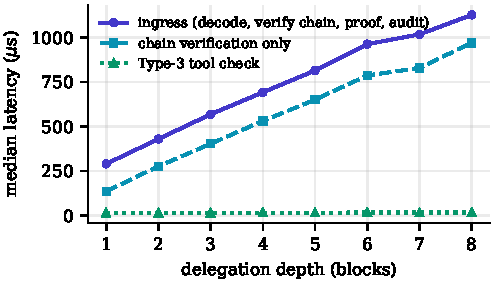
\includegraphics[width=\columnwidth]{figures/latency.pdf}
\caption{Median ingress cost per message versus chain depth (\resCpu, 8 vCPU, Python 3.12). Verification is about one Ed25519 check per block.}
\label{fig:latency}
\end{figure}

\paragraph{Overhead.} Figure~\ref{fig:latency} and Table~\ref{tab:latency} (appendix) report medians over 2{,}000 iterations. Full ingress (chain, proof, replay cache, audit append) takes \resIngressOne~$\mu$s at depth~1 and \resIngressThree~$\mu$s at depth~3, growing linearly at about one signature verification per block. The Type-3 check is \resToolUs~$\mu$s, against \resBearerUs~$\mu$s for an HMAC bearer check. A complete guarded NLIP round trip over \code{nlip\_server} with a three-block chain costs \resHttpGuarded~ms against \resHttpPlain~ms unguarded (in-process ASGI, so excluding network time). That is small next to the seconds an LLM call takes. Warrants are \resWarrantOne~B at depth~1 and \resWarrantThree~B at depth~3.

\section{Discussion and Limitations}
\emph{Deterministic agents.} We evaluate against the worst case, an agent that follows every injected instruction, rather than a specific LLM. \sys{}'s guarantees do not depend on the model, but utility under real LLM planners (e.g.\ AgentDojo tasks~\cite{agentdojo}) is future work. \emph{Budgets are local}: each gateway's ledger bounds spending through \emph{that} gateway. Budgets spanning several services need a shared ledger or escrow. \emph{Revocation freshness} depends on how revocations reach verifiers. We provide in-memory and SQLite stores; gossip or a revocation endpoint is needed in deployment. \emph{Key distribution} and rotation are out of scope (Area~02). \emph{Structured tool arguments} are required: a tool that takes free text cannot be constrained by caveats. \emph{Clock skew} is tolerated up to a 5\,s leeway plus the 60\,s proof window. \emph{Privacy}: warrants reveal the delegation chain (key ids, caveats) to every downstream agent; selective disclosure would need different cryptography. \emph{Policy language}: caveats are deliberately simple. Richer conditions would need a Datalog like Biscuit's~\cite{biscuit}, at the cost of analysability.

\section{Related Work}
\sys{} applies capability thinking~\cite{saltzer1975,hardy1988} to NLIP. SPKI/SDSI~\cite{rfc2693} introduced signed delegation chains with monotone tags. Macaroons~\cite{macaroons} added contextual caveats with HMAC chaining; Biscuit~\cite{biscuit} and UCAN~\cite{ucan} offer public-key attenuable tokens. We adopt their attenuation model but specialise caveats for agent payments, bind each use to an NLIP message and audience, cascade revocation along lineage, and integrate enforcement at ECMA-434 control points. OAuth token exchange~\cite{rfc8693} and DPoP~\cite{rfc9449} provide per-hop narrowing and sender binding but need an online authorisation server and cannot express amounts or payees. South et al.~\cite{south2025} extend OAuth/OpenID Connect with agent-specific delegation credentials; we provide an offline-verifiable, standard-grounded instantiation with a measured attack suite. CaMeL~\cite{camel} uses capabilities \emph{inside} one agent to stop injected data from steering control flow. \sys{} is complementary: it limits what any agent can do \emph{across} agents.

\section{Conclusion}
\sys{} makes delegated authority in NLIP systems explicit, narrowable, bound to each message, revocable and auditable, using only boundary-visible data. It blocks all 14 attack classes we tested with no false refusals at sub-millisecond cost. Code, attack suite, dashboard and reproduction scripts: \url{https://github.com/onepolymath/nlip-warrant}.

\bibliographystyle{ACM-Reference-Format}
\bibliography{refs}

\appendix
\needspace{10\baselineskip}
\section{Verification Algorithm}\label{app:alg}
\begin{lstlisting}
verify(W = [b0..bn], now):
  n+1 <= MAX_DEPTH;  b0.iss in trusted_roots;  b0.parent = null
  eff := b0.caveats
  for i in 0..n:
    Ed25519.verify(bi.iss, "nlip-warrant/v1/block\0" || canon(bi.payload), bi.sig)
    if i > 0:
      bi.parent = sha256(canon(b(i-1)));  bi.iss = b(i-1).sub
      [bi.nbf, bi.exp] within [b(i-1).nbf, b(i-1).exp]
      narrowing_violations(eff, bi.caveats) = {}   # else attenuation_widened
      eff := meet(eff, bi.caveats)
    bi.nbf - leeway <= now < bi.exp + leeway
  no block bk revoked by any issuer of b0..bk
  return eff
ingress(msg): W, P := tokens(msg); eff := verify(W)
  signer := (W.leaf.sub = me) ? W.leaf.iss : W.leaf.sub
  me.aud in eff.audiences;  verify(P, signer, leaf_id(W), me.aud,
     sha256(canon(msg minus proofs)), |now - P.ts| <= 60s, P.nonce fresh)
\end{lstlisting}

\section{Mapping to ECMA-434 SCOs}\label{app:sco}
\begin{table}[h]
\caption{ECMA-434 security countermeasures served by \sys{}.}
\small
\begin{tabular}{@{}p{2.2cm}p{5.6cm}@{}}
\toprule
SCO & \sys{} mechanism \\
\midrule
7.2.1 Client authN & Proof of possession by the sender's Ed25519 key \\
7.2.2 Client authZ & Chain verification at ingress; Type-3 check before every tool call \\
7.2.3 Privilege misuse & Meet of all grants; explicit narrowing; purpose and payee caveats \\
7.2.4 Traceability, cost & Hash-chained signed logs keyed by root/leaf id; cumulative budgets \\
7.2.5 DoS & Early fail-closed rejection; 16\,KiB warrant limit; depth cap; issuer-only revocation \\
7.3.1 Prompt injection & Injected tool calls outside the grant are refused (impact containment) \\
7.3.2 Runtime controls & Time-of-use expiry/revocation checks; per-call caps \\
\bottomrule
\end{tabular}
\end{table}

\section{Latency Breakdown}
\begin{table}[h]
\caption{Median cost by chain depth (2{,}000 iterations).}
\label{tab:latency}
\small
\begin{tabular}{@{}rrrrr@{}}
\toprule
Depth & Warrant (B) & Verify ($\mu$s) & Ingress ($\mu$s) & Tool ($\mu$s) \\
\midrule
1 & 605 & 134 & 289 & 12 \\
2 & 1{,}114 & 276 & 429 & 13 \\
3 & 1{,}623 & 402 & 569 & 13 \\
4 & 2{,}133 & 531 & 693 & 14 \\
6 & 3{,}151 & 788 & 964 & 15 \\
8 & 4{,}170 & 972 & 1129 & 15 \\
\bottomrule
\end{tabular}

\end{table}

\section{Reproduction}
\begin{lstlisting}
git clone https://github.com/onepolymath/nlip-warrant && cd nlip-warrant
make install          # uv sync (Python 3.11+)
make test             # 138 tests, coverage gate 95%
make demo             # three-agent NLIP scenario over HTTP
make eval bench report  # every table and figure in this paper
\end{lstlisting}
All numbers in this paper are generated by \code{make report} from \code{eval/results/*.json} into \code{paper/generated/}.
\end{document}
